\documentclass[11pt]{article}
\usepackage[margin=1in]{geometry}
\usepackage{graphicx}
\usepackage{amsmath}
\usepackage{amssymb}
\usepackage{multirow}

\title{The Gosset Aesthetic: Why the Exceptional Series Ends at $E_8$}
\author{A visual argument through Coxeter-plane projections}
\date{}

\begin{document}
\maketitle

\section*{The Question}

Thorold Gosset (1869--1929), an artist and lawyer, systematically studied
semiregular polytopes in higher dimensions around 1900. Among his discoveries
were the polytopes $2_{21}$, $3_{21}$, and $4_{21}$ in dimensions 6, 7, and 8,
with 27, 56, and 240 vertices respectively.

These polytopes correspond precisely to the exceptional Lie groups $E_6$, $E_7$,
and $E_8$---a connection fully understood only decades later through the
development of root system theory and Coxeter groups. But could Gosset, working
visually and geometrically, have sensed that \textbf{$E_8$ was the natural
endpoint} of something special, even without the formal Lie algebra machinery?

We explore this through Coxeter-plane projections of the polytope edge graphs.

\section*{The Classical Series: $D_n$ (predictable, infinite)}

The $D$-series of polytopes (demihypercubes) form an infinite classical family.
Each has predictable structure:

\begin{figure}[h!]
\centering
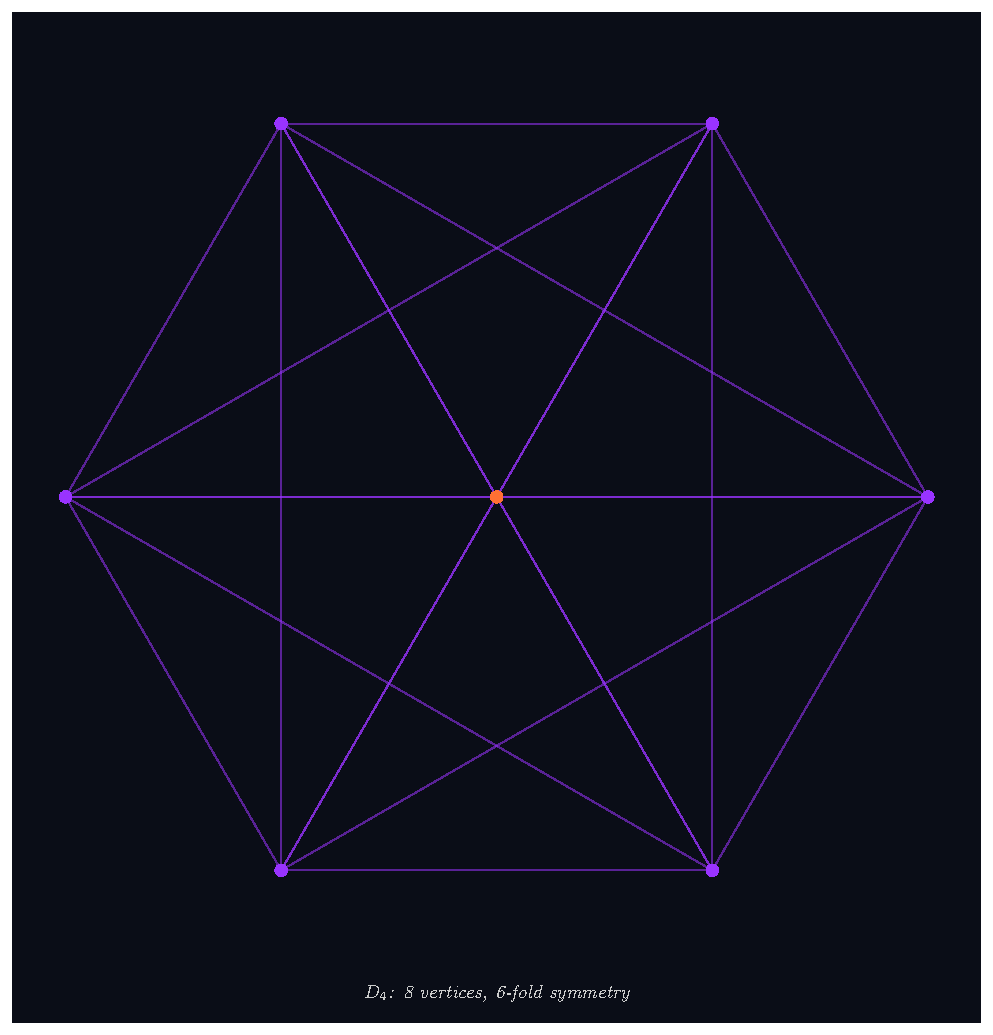
\includegraphics[width=0.3\textwidth]{d4_graph.pdf}
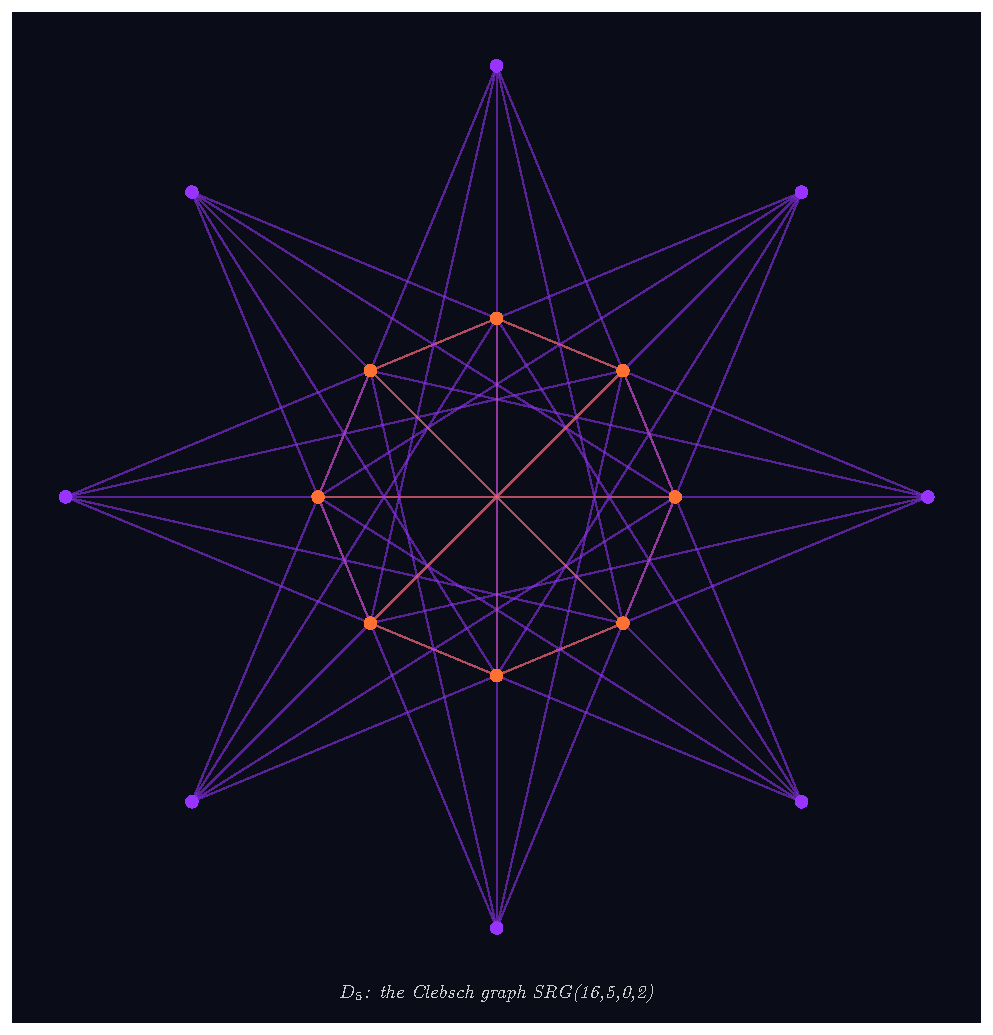
\includegraphics[width=0.3\textwidth]{e5_clebsch.pdf}
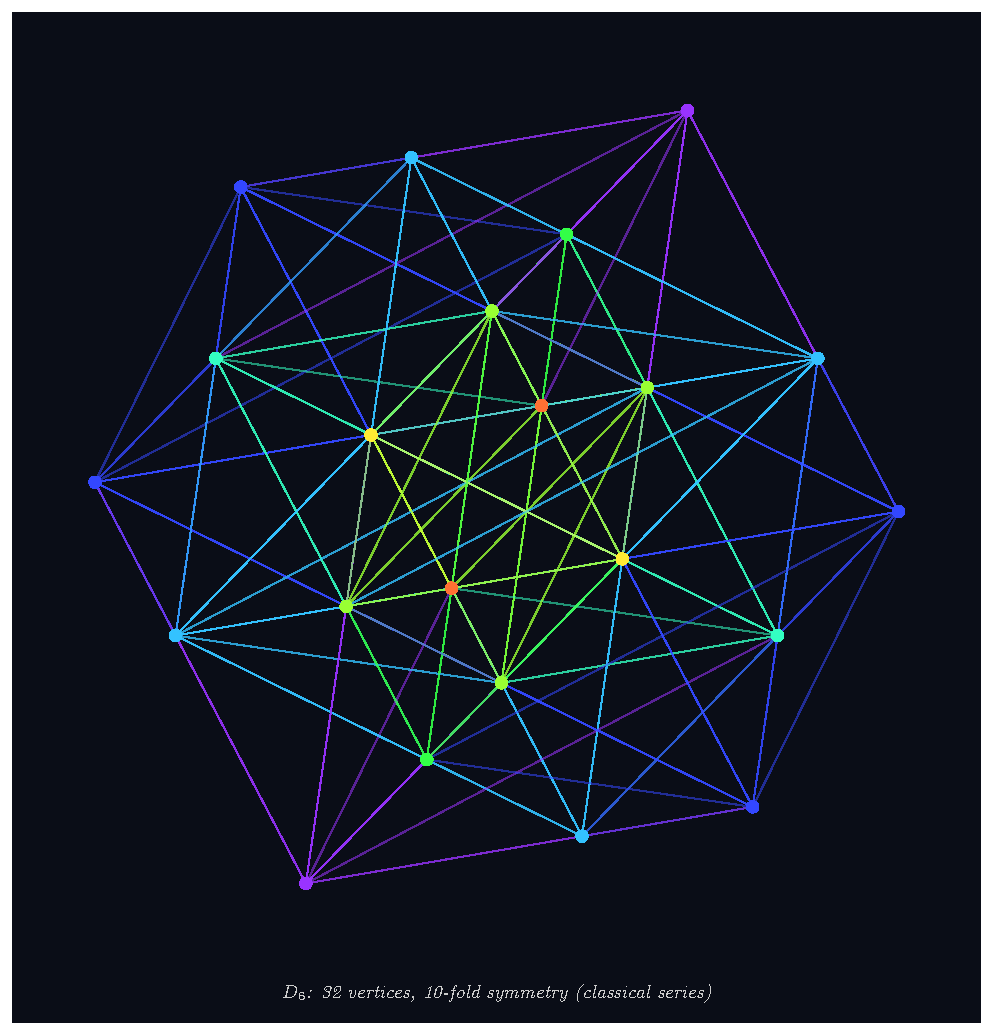
\includegraphics[width=0.3\textwidth]{d6_graph.pdf}
\caption{The D-series: $D_4$ (8 vertices, 6-fold), $D_5$ (16 vertices, 8-fold),
$D_6$ (32 vertices, 10-fold). Vertices double, symmetry increases by 2 each time.
The pattern is \textbf{regular and predictable}.}
\end{figure}

\textbf{Pattern:} $D_n$ has $2^{n-1}$ vertices, Coxeter number $h = 2n-2$.
\begin{itemize}
\item $D_4$: 8 vertices, $h=6$
\item $D_5$: 16 vertices, $h=8$
\item $D_6$: 32 vertices, $h=10$
\item $D_7$: 64 vertices, $h=12$ (would look similar)
\item $\ldots$ continues forever
\end{itemize}

\clearpage

\section*{The Exceptional Series: $E_6 \subset E_7 \subset E_8$ (special, finite)}

The exceptional polytopes have an entirely different quality:

\begin{figure}[h!]
\centering
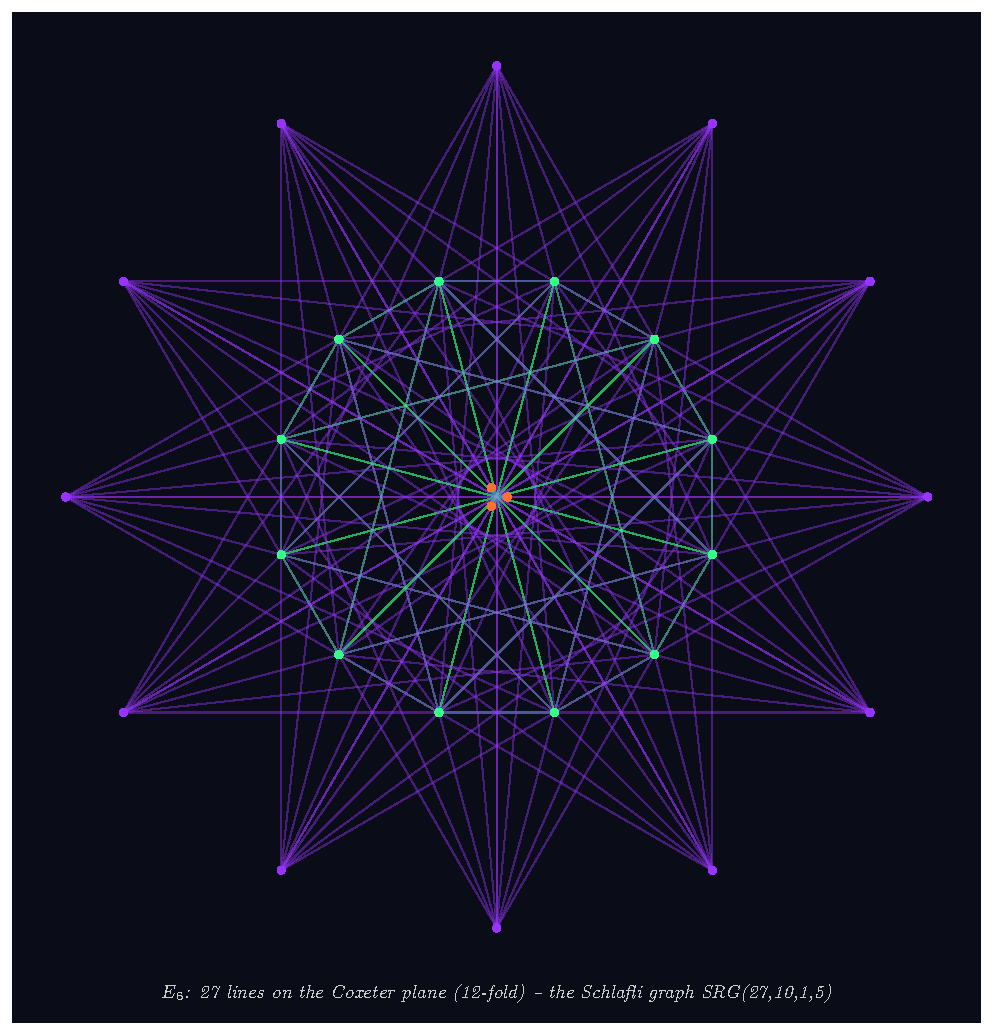
\includegraphics[width=0.3\textwidth]{e6_schlafli.pdf}
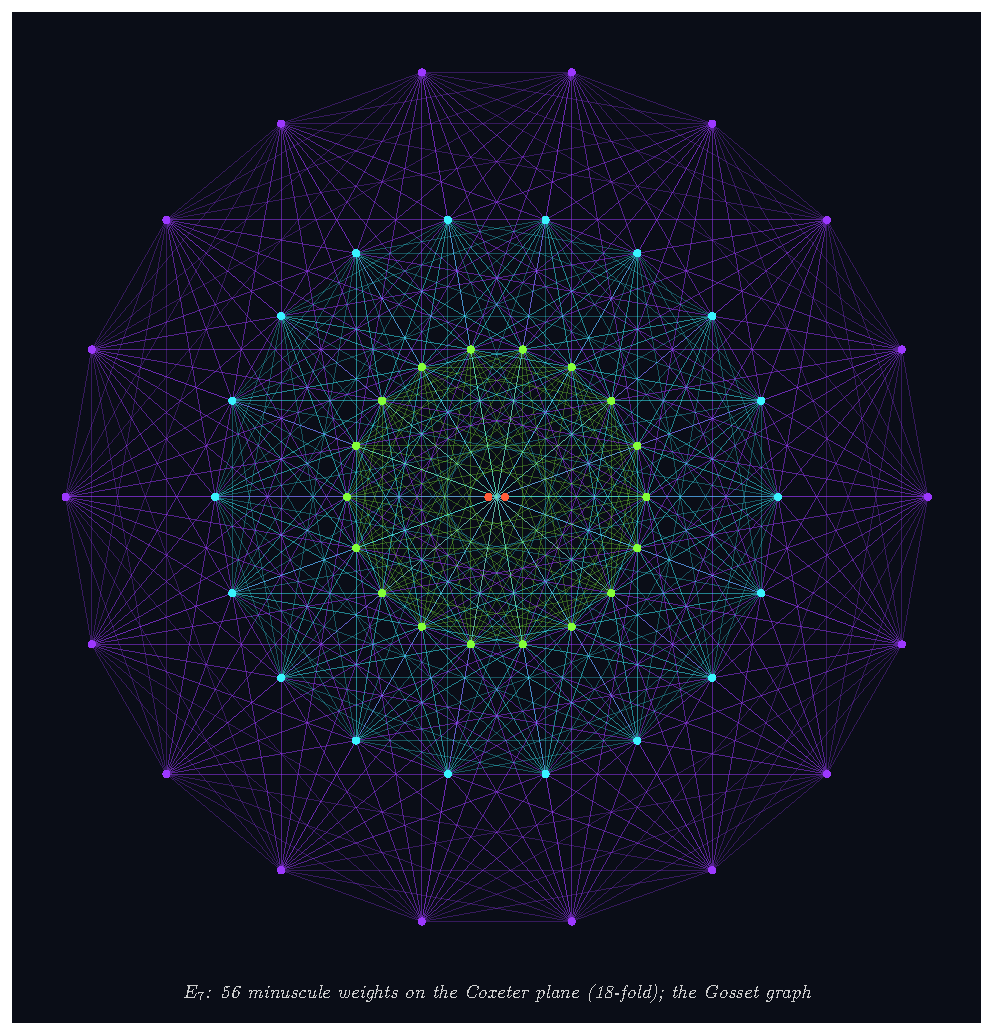
\includegraphics[width=0.3\textwidth]{e7_mandala.pdf}
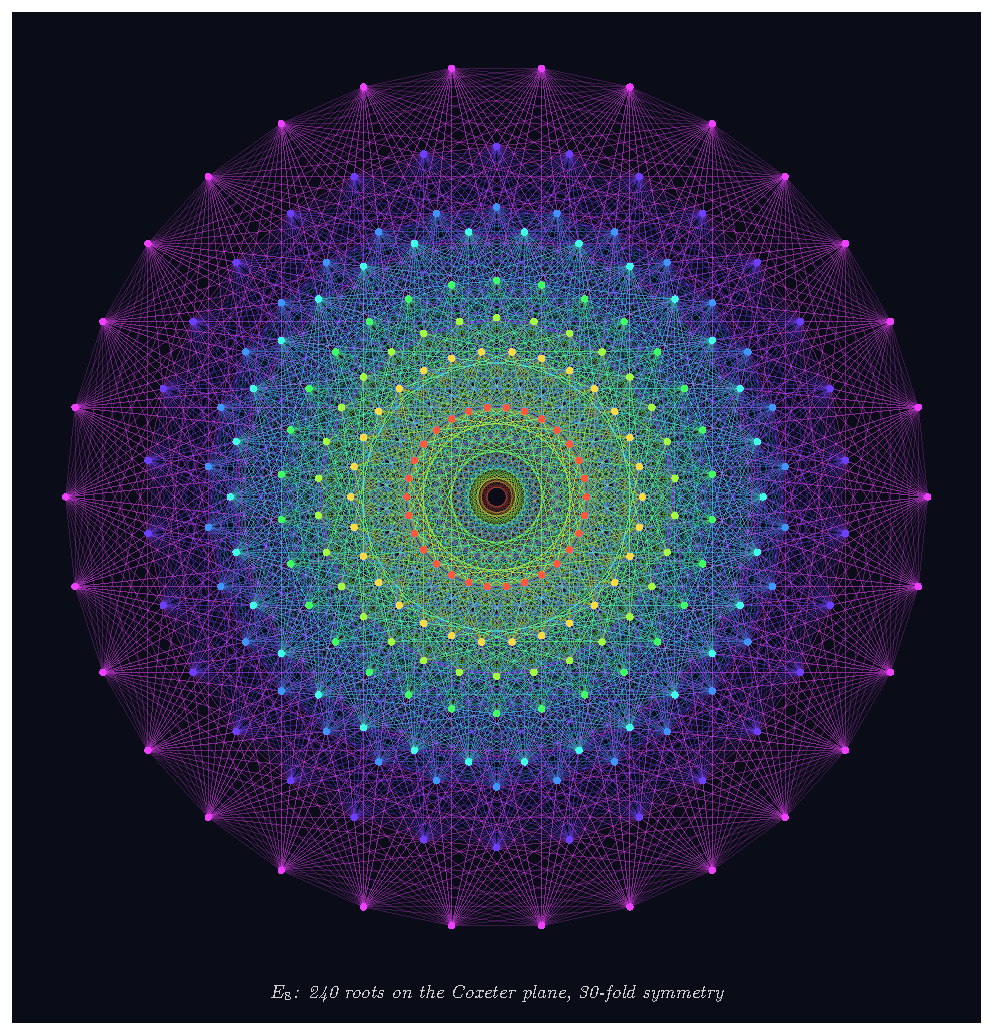
\includegraphics[width=0.26\textwidth]{e8_mandala.pdf}
\caption{The exceptional series: $E_6$ (27 vertices, 12-fold), $E_7$ (56 vertices,
18-fold), $E_8$ (240 vertices, 30-fold). Each has unique numerical properties and
\textbf{irreproducible beauty}.}
\end{figure}

\textbf{What's different?}
\begin{itemize}
\item \textbf{Non-doubling vertex counts:} 27, 56, 240 (not powers of 2)
\item \textbf{Irregular symmetry growth:} 12 → 18 → 30 (by factors 1.5, 1.67)
\item \textbf{Increasing visual complexity:} Each more intricate than the last
\item \textbf{``Magical'' numbers:} 27 lines on a cubic surface, 28 bitangents, 240 kissing number in 8D
\item \textbf{Perfect interlocking:} $E_6 \subset E_7 \subset E_8$ as nested structures
\end{itemize}

\section*{What Happens Beyond $E_8$?}

There is no $E_9$. The polytope $5_{21}$ exists (in 9D, related to $D_5$ structures),
but it \textbf{reverts to classical patterns}---it looks like ``more $D$-series,''
not a continuation of the exceptional quality.

\begin{figure}[h!]
\centering
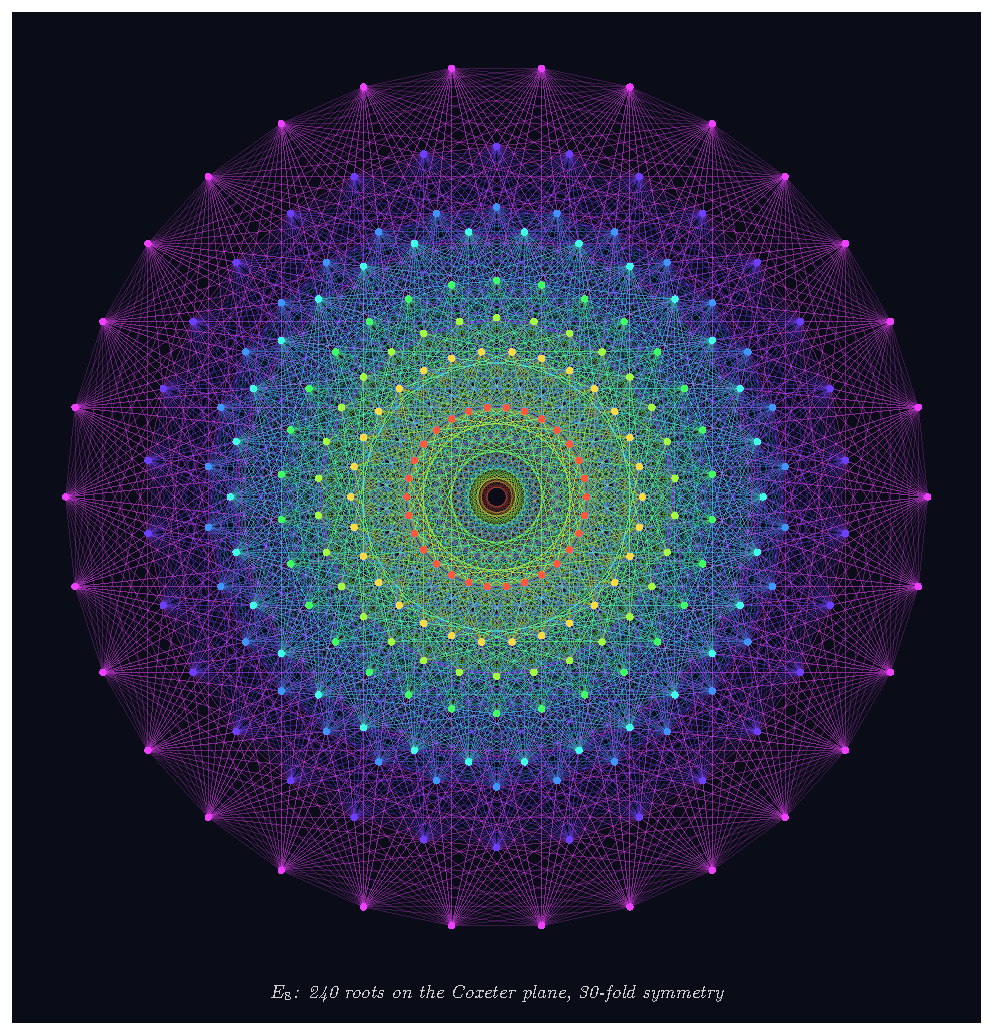
\includegraphics[width=0.35\textwidth]{e8_mandala.pdf}
\hspace{0.5cm}
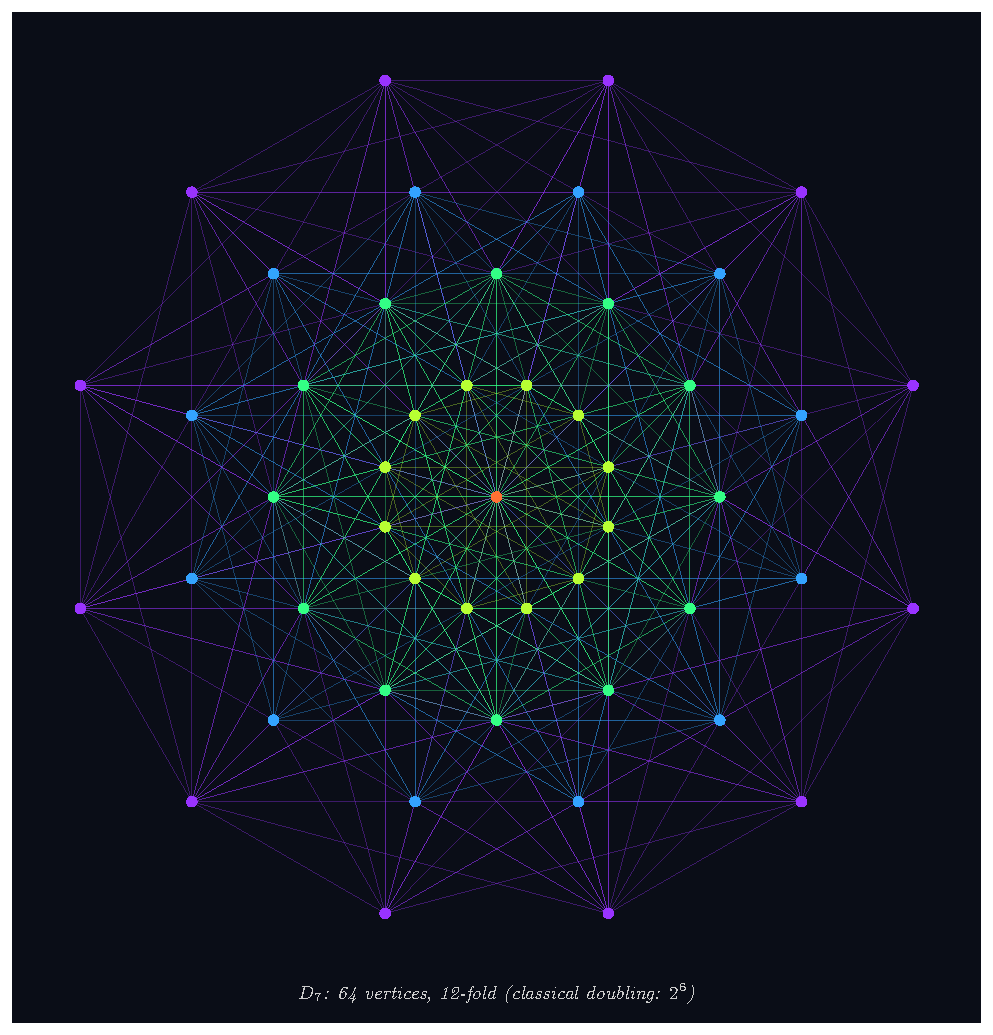
\includegraphics[width=0.35\textwidth]{d7_classical.pdf}
\caption{The endpoint: \textbf{E8} (240 vertices, 30-fold, exceptional) vs \textbf{D7}
(64 = $2^6$ vertices, 12-fold, classical). Beyond E8, the natural continuation
is D7, D8, \ldots---returning to predictable power-of-2 patterns. The ``E9'' that might
continue the exceptional series \textbf{does not exist}.}
\end{figure}

\textbf{Key observation:} D7 has the same 12-fold symmetry as E6, but 64 vertices (a power
of 2) instead of 27. The D-series ``shadows'' the E-series in Coxeter number but lacks
the exceptional numerical magic.

\section*{The Aesthetic Argument}

\textbf{What Gosset could have observed visually:}

\begin{enumerate}
\item The \textbf{D-series is infinite and repetitive}---regular doubling, predictable symmetry
\item The \textbf{E-series has unique numerical harmony}---27, 56, 240 feel ``complete''
\item \textbf{$E_8$ has maximal richness}---30-fold symmetry, 8 concentric rings,
240 vertices forming the densest sphere packing in 8D
\item \textbf{Beyond $E_8$, the pattern breaks}---no $E_9$ with comparable special properties;
$5_{21}$ and beyond look classical
\end{enumerate}

An artist working with these forms might sense: ``$E_8$ is the culmination.
Something closes here.''

\vspace{1em}

\textbf{The formal answer} (discovered later): The classification of simple Lie
algebras shows precisely 5 exceptional types: $G_2$, $F_4$, $E_6$, $E_7$, $E_8$.
There is no $E_9$ because the Dynkin diagram would require angles that don't close
into a finite reflection group.

But Gosset, drawing these polytopes by hand, may have \textbf{seen this truth
geometrically before it could be proven algebraically}.

\section*{Summary: The Complete Ladder}

\begin{center}
\begin{tabular}{lcccc}
\hline
Type & Vertices & Coxeter $h$ & Polytope & Series \\
\hline
$D_4$ & 8 & 6 & 16-cell & \multirow{4}{*}{Classical (infinite)} \\
$D_5$ & 16 & 8 & demihypercube & \\
$D_6$ & 32 & 10 & demihypercube & \\
$D_7$ & 64 = $2^6$ & 12 & demihypercube & \\
\hline
$E_6$ & 27 & 12 & $2_{21}$ & \multirow{3}{*}{\textbf{Exceptional (finite)}} \\
$E_7$ & 56 & 18 & $3_{21}$ & \\
$E_8$ & \textbf{240} & \textbf{30} & $4_{21}$ & \\
\hline
``$E_9$'' & --- & --- & does not exist & \\
$5_{21}$ & ? & 14 & related to $D_5$ & (classical) \\
\hline
\end{tabular}
\end{center}

\textbf{Notice:} $D_7$ and $E_6$ both have $h=12$, but D7 follows the power-of-2 pattern
while E6 has the exceptional count 27.

The ladder ends at $E_8$ not by accident, but by \textbf{geometric necessity}---a
truth visible in the drawings themselves.

\end{document}
